% !TEX root = ../../../main.tex
% 来源：中学数学实验教材·第三册（高中数学）
% 章节：任意角的三角函数 / 三角函数的诱导公式
% 原始文件：6.tex，行 1872-1900
% 类型：tikz
% ---
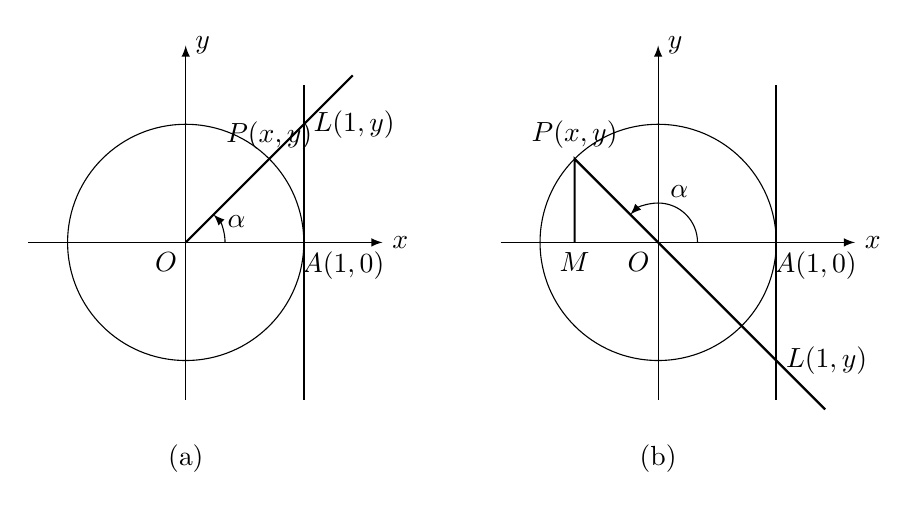
\begin{tikzpicture}[>=latex]
\begin{scope}
\draw[->](-2,0)--(2.5,0)node[right]{$x$};
\draw[->](0,-2)--(0,2.5)node[right]{$y$};
\draw (0,0) circle(1.5);
\draw[thick] (1.5,-2)--(1.5,2);
\node at (-.25,-.25){$O$};
\node at (2,0)[below]{$A(1,0)$};
\draw[thick] (0,0)--(45:3);
\node at (1.5,1.5)[right]{$L(1,y)$};
\node at (45:1.5)[above]{$P(x,y)$};
\draw[->] (.5,0) arc (0:45:.5);
\node at (45/2:.7) {$\alpha$};
\node at (0,-2.75){(a)};
\end{scope}
\begin{scope}[xshift=6cm]
\draw[->](-2,0)--(2.5,0)node[right]{$x$};
\draw[->](0,-2)--(0,2.5)node[right]{$y$};
\draw (0,0) circle(1.5);
\draw[thick] (1.5,-2)--(1.5,2);
\node at (-.25,-.25){$O$};
\node at (2,0)[below]{$A(1,0)$};
\draw[thick] (-1.5/1.414,0)node[below]{$M$}--(90+45:1.5)node[above]{$P(x,y)$}--(0,0)--(-45:3);
\node at (1.5,-1.5)[right]{$L(1,y)$};
\draw[->] (.5,0) arc (0:45+90:.5);
\node at (135/2:.7){$\alpha$};
\node at (0,-2.75){(b)};
\end{scope}
\end{tikzpicture}
